 

\documentclass{beamer} %
\usepackage{beamerthemesplit} % new 
\usepackage[utf8]{inputenc}

\usetheme{Boadilla}


\makeatother
\setbeamertemplate{footline}
{
  \leavevmode%
  \hbox{%
  \begin{beamercolorbox}[wd=.4\paperwidth,ht=2.25ex,dp=1ex,center]{author in head/foot}%
    \usebeamerfont{author in head/foot}\insertshortauthor
  \end{beamercolorbox}%
  \begin{beamercolorbox}[wd=.6\paperwidth,ht=2.25ex,dp=1ex,center]{title in head/foot}%
    \usebeamerfont{title in head/foot}Classe Ibrida per l'Algebra Lineare.\hspace*{3em}
    \insertframenumber{} / \inserttotalframenumber\hspace*{1ex}
  \end{beamercolorbox}}%
  \vskip0pt%
}
\makeatletter



\usefonttheme{professionalfonts}
\usepackage{times}
\usepackage{tikz}
\usepackage{amsmath}
\usepackage{verbatim}
\usetikzlibrary{arrows,shapes,matrix,positioning}

\usepackage{hyperref}

\usepackage{xcolor} %pacchetto per cambiare il colore di simboli nei display math
\usepackage{graphicx}

\usepackage{listings}

%DOPPIA FRECCIA CON COMMENTO
\makeatletter
\newcommand\xleftrightarrow[2][]{%
  \ext@arrow 9999{\longleftrightarrowfill@}{#1}{#2}}
\newcommand\longleftrightarrowfill@{%
  \arrowfill@\leftarrow\relbar\rightarrow}
\makeatother

%tabelline
\definecolor{redi}{RGB}{255,38,0}
\definecolor{redii}{RGB}{200,50,30}
\definecolor{yellowi}{RGB}{255,251,0}
\definecolor{bluei}{RGB}{0,150,255}
\definecolor{blueii}{RGB}{135,247,210}
\definecolor{blueiii}{RGB}{91,205,250}
\definecolor{blueiv}{RGB}{115,244,253}
\definecolor{bluev}{RGB}{1,58,215}
\definecolor{orangei}{RGB}{240,143,50}
\definecolor{yellowii}{RGB}{222,247,100}
\definecolor{greeni}{RGB}{166,247,166}


\tikzset{ 
table/.style={
  matrix of nodes,
  row sep=-\pgflinewidth,
  column sep=-\pgflinewidth,
  nodes={rectangle,draw=black,text width=1.25ex,align=center},
  text depth=0.25ex,
  text height=1ex,
  nodes in empty cells
  },
texto/.style={font=\footnotesize\sffamily},
title/.style={font=\small\sffamily}
}


\newcommand\CellText[2]{%
  \node[texto,left=of mat#1,anchor=east]
  at (mat#1.west)
  {#2};
}

\newcommand\SlText[2]{%
  \node[texto,left=of mat#1,anchor=west,rotate=75]
  at ([xshift=3ex]mat#1.north)
  {#2};
}

\newcommand\RowTitle[2]{%
\node[title,left=6.3cm of mat#1,anchor=west]
  at (mat#1.north west)
  {#2};
}



\begin{document}
\title{Implementazione di un modulo per il calcolo del determinante in una libreria ibrida per l'Algebra Lineare.} 
\author{Antonio Miti} 
\date{\today} 
\frame{\titlepage} 

%\frame{\frametitle{Table of contents}\tableofcontents} 
% For every picture that defines or uses external nodes, you'll have to
% apply the 'remember picture' style. To avoid some typing, we'll apply
% the style to all pictures.
\tikzstyle{every picture}+=[remember picture]

% By default all math in TikZ nodes are set in inline mode. Change this to
% displaystyle so that we don't get small fractions.
\everymath{\displaystyle}



\section{Progetto iniziale} 
\subsection{Concetti chiave:}
\begin{frame}{Progetto iniziale}{Concetti chiave:} 
	\begin{columns}
		\begin{column}{3.5cm}
\begin{tabular}{l l l}
\uncover<1->{$\left[ A \right]_{\mbox{\tiny device}}$ &  & $\left[ A \right]_{\mbox{\tiny host}}$ \\ }
\uncover<2->{$ \Downarrow $ &  & $ \Downarrow $ \\  
$\left[ A' \right]_{\mbox{\tiny device}}$ &  & $\left[ A' \right]_{\mbox{\tiny host}}$ \\ }
\uncover<3->{$ \Downarrow $ &  & $ \Downarrow $ \\  
$ \vdots $ &  & $ \vdots $ \\
$ \Downarrow $ &  & $ \Downarrow $ \\
$\left[ A'' \right]_{\mbox{\tiny device}}$} & \uncover<4->{ $ \xleftrightarrow{\text{\tiny sync}}$}  &\uncover<3->{ $\left[ A'' \right]_{\mbox{\tiny host}}$ }\\ 
\end{tabular} 

		\end{column}

		\begin{column}{6.5cm}
			\begin{itemize}
				\item<1-> 2 copie della matrice, una memorizzata sull'host e l'altra su device. \tiny (Memorizzate come array 1d di \emph{float}.) 
				\item<2-> 2 copie di ciascun metodo.
				\item<3-> Possibilita' di effettuare calcoli complessi separatamente sul solo host o sul device.
				\item<4-> Metodi per sincronizzare le 2 copie della matrice. \tiny (Per minimizzare il trasferimento dei dati fra host e device.) 
			\end{itemize}
		\end{column}

	\end{columns}


\end{frame}


\subsection{Il codice}
\begin{frame}[fragile] {Progetto iniziale} {il codice}
   \lstset{language=C++,
           basicstyle=\ttfamily\scriptsize,
           keywordstyle=\color{blue}\ttfamily,
           stringstyle=\color{red}\ttfamily,
           commentstyle=\color{green}\ttfamily,
          breaklines=true
          }
\begin{itemize}


\item L'oggetto principale della libreria è costituito dalla classe \href{run:/home/tony/CudaCorso/ProgettoFinale/CudaMatrixClass/Src/Cuda_FloatMatrixClass.cuh}{\color{red}  \emph{matrice}}.
\begin{lstlisting}
class matrice{
	float *A_host ;		// puntatore alle variabli host
	float *A_dev ; 		//puntatori alle variabli device
	unsigned int ROW,COL,N;

	bool flagCuda;		// flag presenza di scheda cuda
	bool flagMemory;	// flag di sincronizzazione copia host -device
	bool flagSquare; 	//flag matrice quadrata
[...]
\end{lstlisting}\pause 

\item  Il sorgente di ogni modulo è salvato in header file distinti.\pause 

\item Anche i singoli CUDA kernel utilizzati sono salvati in specifici header.\pause 

\item ... il modulo che verrà analizzato sarà quello di \href{run:/home/tony/CudaCorso/ProgettoFinale/CudaMatrixClass/Src/Condensation.cuh}{\color{red}  \emph{"condensazione"}}.

\end{itemize}
\end{frame}


\section{Algoritmi di condensazione}
\subsection{L'idea}
\begin{frame}{Algoritmi di condensazione}{L'idea}
Classe di algoritmi pensata esplicitamente per il calcolo dei determinanti.
Basata sulla tesi:
\begin{displaymath}
\exists \mbox{T}: \mbox{ Mat}(n,n) \rightarrow \mbox{ Mat}(n 1,n-1)
\end{displaymath}
tale che
\begin{displaymath}
 \forall A \in \mbox{ Mat}(n,n)\quad \exists P_{(A)} \in \mathbb{K}\: \qquad |\quad  \mbox{det}(A) =  P_{(A)} \cdot \mbox{det}\big( \mbox{T}(A) \big)
\end{displaymath}\pause
\vspace{1cm}
$B= \mbox{T}(A)$ è detta \emph{condensazione} della matrice.

\end{frame}


\begin{frame}{Algoritmi di condensazione}{L'idea}
\tikzstyle{na} = [baseline=-.5ex]
L'applicazione consecutiva di tale operatore ...
\begin{displaymath}
	\cdots
		\left[ \begin{array}{ccc} a_{00} & a_{01} & a_{02} \\ a_{10} & a_{11} & a_{12} \\ a_{20} & a_{21} & a_{22}  \end{array} \right] 
\uncover<2->{
	\tikz[baseline]{ \node[fill=blue!20,anchor=base] (n1){$ \mapsto$}; }
		\left[ \begin{array}{cc} \color{blue}b_{00} & \color{blue}b_{01} \\ \color{blue}b_{10} & \color{blue}b_{11}  \end{array} \right] 
}
\uncover<3->{
	\tikz[baseline]{ \node[fill=blue!20,anchor=base] (n2){$ \mapsto$}; }
		\left[ \begin{array}{c} \tikz[baseline]{ \node[fill=green!20,anchor=base] (n3){$ D$}; }   \end{array} \right] 
}
\end{displaymath}
\newline
\begin{displaymath}
\uncover<5->{\mbox{det}(A_{1})= \cdots}	\uncover<2->{\tikz[baseline]{ \node[fill=blue!20,anchor=base] (t1){$ P_{(A_{n-3})}$}; }} \uncover<5->{\cdot} \uncover<3->{\tikz[baseline]{ \node[fill=blue!20,anchor=base] (t2){$ P_{(A_{n-2})}$}; }} \uncover<5->{\cdot}\uncover<4->{ \tikz[baseline]{ \node[fill=blue!20,anchor=base] (t3){$ D$}; }}
\end{displaymath}
\uncover<5->{Permette di calcolare il determinante della matrice come prodotto dei \emph{Pivot}.}

% Now it's time to draw some edges between the global nodes. Note that we
% have to apply the 'overlay' style.
\begin{tikzpicture}[overlay]
       \path[->]<2-> (n1) edge [out=-90, in=90] (t1);
       \path[->]<3-> (n2) edge [out=-90, in=90] (t2);
       \path[->]<4-> (n3) edge [out=-90, in=90] (t3);
\end{tikzpicture}

\end{frame}

\subsection{La formula di Salem-Said}
\begin{frame}[fragile]{Algoritmi di condensazione}{La formula di Salem-Said}
 
	\begin{columns}
		\begin{column}{4cm}
    
    \begin{tikzpicture}
        \matrix [matrix of math nodes,left delimiter=(,right delimiter=)] (m)
        {
            \cdots & a_{0j} & \cdots & \color{red}a_{0l} &\cdots \\
            		 & \vdots &  & \vdots &  \\ 
			\cdots & \color{blue}a_{ij} & \cdots & a_{il}  & \\
			& \vdots &  & \; \vdots \; & \ddots \\
        };  
	  \uncover<1>{ \draw[color=red] (m-1-4.north west) -- (m-1-4.north east) -- (m-1-4.south east) -- (m-1-4.south west) -- (m-1-4.north west);}
      \uncover<2->{ \draw[color=red] (m-1-1.north west) -- (m-1-5.north east) -- (m-1-5.south east) -- (m-1-1.south west) -- (m-1-1.north west);}
      \uncover<2->{\draw[color=red] (m-1-4.north west) -- (m-1-4.north east) -- (m-4-4.south east) -- (m-4-4.south west) -- (m-1-4.north west);}
      \uncover<3->{\draw[color=blue] (m-1-2.north west) -- (m-1-2.north east) -- (m-1-2.south east) -- (m-1-2.south west) -- (m-1-2.north west);}
      \uncover<3->{\draw[color=blue] (m-1-4.north west) -- (m-1-4.north east) -- (m-1-4.south east) -- (m-1-4.south west) -- (m-1-4.north west);}
      \uncover<3->{\draw[color=blue] (m-3-2.north west) -- (m-3-2.north east) -- (m-3-2.south east) -- (m-3-2.south west) -- (m-3-2.north west);}
      \uncover<3->{\draw[color=blue] (m-3-4.north west) -- (m-3-4.north east) -- (m-3-4.south east) -- (m-3-4.south west) -- (m-3-4.north west);}

    \end{tikzpicture}    

\begin{displaymath}
\Downarrow \mbox{T}_{\mbox{\tiny SS}}
\end{displaymath}

	\begin{tikzpicture}
	 \matrix [matrix of math nodes,left delimiter=(,right delimiter=)] (B)
        {
            \ddots & \vdots &  \\
            		 & b_{i-1,j} &    \\ 
			& \vdots &   \ddots \\
        };  
	\end{tikzpicture}    
    
\begin{tikzpicture}[overlay]
      \uncover<4->{ \path[->]<1-> (m-1-2.south west) edge [bend right] (B-2-2.north west);}
      \uncover<4->{ \path[->]<1-> (m-1-4.south east) edge [bend left] (B-2-2.north east);}
      \uncover<4->{ \path[->]<1-> (m-3-2.south west) edge [bend right] (B-2-2.north west);} 
      \uncover<4->{ \path[->]<1-> (m-3-4.south east) edge [bend left] (B-2-2.north east);} 
      \uncover<4->{\draw[color=blue] (B-2-2.north west) -- (B-2-2.north east) -- (B-2-2.south east) -- (B-2-2.south west) -- (B-2-2.north west);}            

\end{tikzpicture}

		\end{column}

		\begin{column}{6cm}
		Routine di singola condensazione:
			\begin{enumerate}
				\item<1-> Scelta elemento Pivot. \tiny (primo elemento non nullo nella prima riga) 
				\item<2-> Scorro gli elementi. \tiny (nella matrici privata della riga e colonna del pivot)
				\item<3-> Calcolo determinante 2x2 evidenziato.
				\item<4-> Elemento della matrice trasformata = determinante appena calcolato 
			\end{enumerate}
		\uncover<5->{
		Risulta la seguente espressione per $ P_{(A)} = \dfrac{1}{(a_{0l})^{n-2}} $
		}

		\end{column}

	\end{columns}

\end{frame}




\subsection{L'algoritmo modificato.}
\begin{frame}[fragile]{Algoritmi di condensazione}{Versione modificata}


	\begin{columns}
		\begin{column}{4cm}
    
    \begin{tikzpicture}[thick,scale=0.9, every node/.style={scale=0.7}]
        \matrix [matrix of math nodes,left delimiter=(,right delimiter=)] (m)
        {
            \only<1-3>{a_{0,0}} & \only<1-3>{\cdots} & \only<1-2>{ a_{0,l}}\only<3>{a_{0,n-1}}\only<4->{\vdots} & \only<1-3>{\cdots} &  \only<1-2>{ a_{0,n-1}}\only<3>{a_{0,l}}\only<4->{\color{red}\vdots} \\
            	\only<1-3>{\vdots}\only<4->{\dots}	 &  &  \only<1-3>{\vdots} \only<4->{\color{blue}a'_{i,j}} & & \only<1-3>{\vdots} \only<4->{\color{red}a'_{i,n-1}} \\ 
            	\only<1-3>{\vdots}	 &  & \vdots & & \only<1-3>\vdots\only<4->{\color{red}\vdots} \\ 
			\only<1>{a_{n-1,0}}\only<2-3>{\dfrac{a_{n-1,0}}{a_{n-1,l}}}\only<4->{\color{red}\cdots} & \only<1-3>{\cdots} & \only<1>{a_{n-1,l}}\only<2>{1}\only<3>{\dfrac{a_{n-1,n-1}}{a_{n-1,l}}}\only<4->{\color{red}a'_{n-1,i}} & \only<1-3>\cdots\only<4->{\color{red}\cdots} & \only<1>{a_{n-1,n-1}}\only<2>{\dfrac{a_{n-1,n-1}}{a_{n-1,l}}}\only<3>{1}\only<4->{\color{red}1} \\
        };  
    \end{tikzpicture}    
  
      \begin{tikzpicture}[overlay]
	  \uncover<1-2>{ \draw[color=red] (m-4-3.north west) -- (m-4-3.north east) -- (m-4-3.south east) -- (m-4-3.south west) -- (m-4-3.north west);}
	  \uncover<3->{ \draw[color=red] (m-4-5.north west) -- (m-4-5.north east) -- (m-4-5.south east) -- (m-4-5.south west) -- (m-4-5.north west);}
	  \uncover<5->{ \draw[color=blue] (m-4-3.north west) -- (m-4-3.north east) -- (m-4-3.south east) -- (m-4-3.south west) -- (m-4-3.north west);}
	  \uncover<5->{ \draw[color=blue] (m-2-3.north west) -- (m-2-3.north east) -- (m-2-3.south east) -- (m-2-3.south west) -- (m-2-3.north west);}
	  \uncover<5->{ \draw[color=blue] (m-2-5.north west) -- (m-2-5.north east) -- (m-2-5.south east) -- (m-2-5.south west) -- (m-2-5.north west);}
	  \uncover<5->{ \draw[color=blue] (m-4-5.north west) -- (m-4-5.north east) -- (m-4-5.south east) -- (m-4-5.south west) -- (m-4-5.north west);}
    \end{tikzpicture}    

\begin{displaymath}
\Downarrow \mbox{T}_{\mbox{\tiny mod}}
\end{displaymath}

	\begin{tikzpicture}[thick,scale=0.9, every node/.style={scale=0.7}]
	 \matrix [matrix of math nodes,left delimiter=(,right delimiter=)] (B)
        {
            \ddots & \vdots &  \\
            		 & b_{i,j} &    \\ 
			& \vdots &   \ddots \\
        };  
	\end{tikzpicture}    
    
\begin{tikzpicture}[overlay]
      \uncover<5->{ \path[->]<1-> (m-2-3.south west) edge [bend right] (B-2-2.north west);}
      \uncover<5->{ \path[->]<1-> (m-2-5.south east) edge [bend left] (B-2-2.north east);}
      \uncover<5->{ \path[->]<1-> (m-4-3.south west) edge [bend right] (B-2-2.north west);} 
      \uncover<5->{ \path[->]<1-> (m-4-5.south east) edge [bend left] (B-2-2.north east);} 
      \uncover<5->{\draw[color=blue] (B-2-2.north west) -- (B-2-2.north east) -- (B-2-2.south east) -- (B-2-2.south west) -- (B-2-2.north west);}            

\end{tikzpicture}


		\end{column}

		\begin{column}{6cm}
		Routine di singola condensazione:
			\begin{enumerate}
				\item<1-> Scelta elemento Pivot. \tiny (Elemento in modulo maggiore nell'ultima riga) 
				\item<2-> Divisione ultima riga per il valore del Pivot. 
				\item<3-> Scambio colonna del pivot con ultima riga.
				\item<4-> Selezione elemento della matrice fin qui trasformata \tiny (privata della riga e colonna del pivot).
				\item<5-> Calcolo dell'elemento condensato come determinante 2x2.
			\end{enumerate}

		\end{column}

	\end{columns}
\end{frame}

\subsection{Vantaggi}
\begin{frame}{Algoritmi di condensazione}{Vantaggi}
\begin{itemize}
\item<1-> In questo caso il valore $P_{(A)}$, necessario per ricostruire il determinante, coincide con il valore del pivot: $P_{(A)}= a_{n-1,l}$.\newline  \tiny ( in quanto viene condensata la matrice $A'$ di pivot pari ad 1 tramite la formula di Salem Said.)

\item<2-> A differenza dell'algoritmo precendente, non c'è rischio di over-flow o under-flow durante il susseguirsi degli step di condensazione.
\end{itemize}
\uncover<3->{
Sia $S\simeq <|a_{\ast}|>$ la taglia della matrice di partenza e $S'$ della matrice condensata. Si ha:
\begin{displaymath}
S'_{\text{\footnotesize SS}} \simeq S^{2}
\end{displaymath}
\begin{displaymath}
S'_{\text{\footnotesize mod}} \simeq S + \alpha S \simeq S
\end{displaymath}
 \tiny( dove $\alpha$ è una quantità di modulo minore di 1).
}
\pause \pause \pause
\begin{block}{\small Attenzione!}\footnotesize Il determinante è definito come sommatoria di permetuzioni di molti elementi! Per calcolare la produttoria dei pivot sarà comunque necessario implementare una classe per gestire numeri di grande esponente. \end{block}
\end{frame}


\section{Implementazione CPU}
\begin{frame}[fragile]{Implementazione CPU}
   \lstset{language=C++,
           basicstyle=\ttfamily\scriptsize,
           keywordstyle=\color{blue}\ttfamily,
           stringstyle=\color{red}\ttfamily,
           commentstyle=\color{green}\ttfamily,
          breaklines=true
          }

Per realizzare il singolo passo di condensazione sono stati realizzati quattro metodi. \href{run:/home/tony/CudaCorso/ProgettoFinale/CudaMatrixClass/Src/Condensation.cuh}{\tiny (nel file \color{red}  \emph{"Condensation.cuh"})}.\pause

\begin{enumerate}
\item Ricerca del pivot.\pause
\item Divisione della riga.\pause
\item Scambio dell'ultima colonna.\pause
\item Condensazione vera e propria.
\end{enumerate}

\begin{lstlisting}
void matrice::Cpu_Step_Condensation_Simple(){
 int newROW = ROW-1;	int newCOL = COL-1;	

 for(int i=0 ; i<newROW ; i++)for(int j=0 ; j<newCOL ; j++)
  A_host[i*newCOL+j] =A_host[i*COL+j]-A_host[i*COL+COL-1]*A_host[(ROW-1)*COL+j];

 ROW=newROW; COL=newCOL;
[...]
\end{lstlisting}\pause 

I quattro vengono accorpati un un quinto metodo che li cicla fino a condensare una data matrice ad un singolo elemento.
\end{frame}

\subsection{analisi}
\begin{frame}[fragile]{Implementazione CPU}{Analisi}
	\begin{columns}
		\begin{column}{4cm}
     \begin{tikzpicture}
        \matrix [matrix of math nodes,left delimiter=(,right delimiter=)] (m)
        {
            \only<1>{a}\only<2-4>{\color{blue} a}\only<5->{\color{green} a'} & \only<1-5>{b}\only<6->{\color{green}b'} & \only<1-6>{c}\only<7->{\color{green}c'} & \only<1-7>{d}\only<8->{\color{green}d'} \\
            \only<1-9>{e}\only<10->{\color{green}e'} & \only<1-10>{f}\only<11->{\color{green}f'} & \only<1-11>{g}\only<12->{\color{green}g'} & \only<1-12>{h}\only<13->{\color{green}h'} \\
            \only<1-13>{i}\only<14->{\color{green}i'} & l & m & n \\    
            o & p & q & r \\
        };  
        
      \uncover<2->{ \draw[color=red] (m-1-4.north west) -- (m-1-4.north east) -- (m-4-4.south east) -- (m-4-4.south west) -- (m-1-4.north west);}
      \uncover<2->{\draw[color=red] (m-4-1.north west) -- (m-4-4.north east) -- (m-4-4.south east) -- (m-4-1.south west) -- (m-4-1.north west);}
      
      \uncover<3>{ \draw[color=blue] (m-1-1.north west) -- (m-1-1.north east) -- (m-1-1.south east) -- (m-1-1.south west) -- (m-1-1.north west);}
      \uncover<3-4>{\draw[color=blue] (m-1-4.north west) -- (m-1-4.north east) -- (m-1-4.south east) -- (m-1-4.south west) -- (m-1-4.north west);}
      \uncover<3-4>{ \draw[color=blue] (m-4-1.north west) -- (m-4-1.north east) -- (m-4-1.south east) -- (m-4-1.south west) -- (m-4-1.north west);}
      \uncover<4>{ \draw[color=green] (m-1-1.north west) -- (m-1-1.north east) -- (m-1-1.south east) -- (m-1-1.south west) -- (m-1-1.north west);}

      \uncover<6>{ \draw[color=blue] (m-1-2.north west) -- (m-1-2.north east) -- (m-1-2.south east) -- (m-1-2.south west) -- (m-1-2.north west);}
      \uncover<6>{\draw[color=blue] (m-1-4.north west) -- (m-1-4.north east) -- (m-1-4.south east) -- (m-1-4.south west) -- (m-1-4.north west);}
      \uncover<6>{ \draw[color=blue] (m-4-2.north west) -- (m-4-2.north east) -- (m-4-2.south east) -- (m-4-2.south west) -- (m-4-2.north west);}		      

      \uncover<7>{ \draw[color=blue] (m-1-3.north west) -- (m-1-3.north east) -- (m-1-3.south east) -- (m-1-3.south west) -- (m-1-3.north west);}
      \uncover<7>{\draw[color=blue] (m-1-4.north west) -- (m-1-4.north east) -- (m-1-4.south east) -- (m-1-4.south west) -- (m-1-4.north west);}
      \uncover<7>{ \draw[color=blue] (m-4-3.north west) -- (m-4-3.north east) -- (m-4-3.south east) -- (m-4-3.south west) -- (m-4-3.north west);}		
      
      \uncover<8>{ \draw[color=green]  (m-1-4.north west) -- (m-1-4.north east) -- (m-1-4.south east) -- (m-1-4.south west) -- (m-1-4.north west);}	
      \uncover<8>{ \draw[color=blue] (m-2-1.north west) -- (m-2-1.north east) -- (m-2-1.south east) -- (m-2-1.south west) -- (m-2-1.north west);}
      \uncover<8>{\draw[color=blue] (m-2-4.north west) -- (m-2-4.north east) -- (m-2-4.south east) -- (m-2-4.south west) -- (m-2-4.north west);}
      \uncover<8>{ \draw[color=blue] (m-4-1.north west) -- (m-4-1.north east) -- (m-4-1.south east) -- (m-4-1.south west) -- (m-4-1.north west);}	

      \uncover<10>{ \draw[color=green] (m-2-1.north west) -- (m-2-1.north east) -- (m-2-1.south east) -- (m-2-1.south west) -- (m-2-1.north west);}
      \uncover<10>{ \draw[color=blue] (m-2-2.north west) -- (m-2-2.north east) -- (m-2-2.south east) -- (m-2-2.south west) -- (m-2-2.north west);}
      \uncover<10>{\draw[color=blue] (m-2-4.north west) -- (m-2-4.north east) -- (m-2-4.south east) -- (m-2-4.south west) -- (m-2-4.north west);}
      \uncover<10>{ \draw[color=blue] (m-4-2.north west) -- (m-4-2.north east) -- (m-4-2.south east) -- (m-4-2.south west) -- (m-4-2.north west);}		
      
      \uncover<11>{ \draw[color=green] (m-2-2.north west) -- (m-2-2.north east) -- (m-2-2.south east) -- (m-2-2.south west) -- (m-2-2.north west);}
      \uncover<11>{ \draw[color=blue] (m-2-3.north west) -- (m-2-3.north east) -- (m-2-3.south east) -- (m-2-3.south west) -- (m-2-3.north west);}
      \uncover<11>{\draw[color=blue] (m-2-4.north west) -- (m-2-4.north east) -- (m-2-4.south east) -- (m-2-4.south west) -- (m-2-4.north west);}
      \uncover<11>{ \draw[color=blue] (m-4-3.north west) -- (m-4-3.north east) -- (m-4-3.south east) -- (m-4-3.south west) -- (m-4-3.north west);}			
      
      \uncover<12>{ \draw[color=green] (m-2-3.north west) -- (m-2-3.north east) -- (m-2-3.south east) -- (m-2-3.south west) -- (m-2-3.north west);}
      \uncover<12>{ \draw[color=blue] (m-3-1.north west) -- (m-3-1.north east) -- (m-3-1.south east) -- (m-3-1.south west) -- (m-3-1.north west);}
      \uncover<12>{\draw[color=blue] (m-3-4.north west) -- (m-3-4.north east) -- (m-3-4.south east) -- (m-3-4.south west) -- (m-3-4.north west);}
      \uncover<12>{ \draw[color=blue] (m-4-1.north west) -- (m-4-1.north east) -- (m-4-1.south east) -- (m-4-1.south west) -- (m-4-1.north west);}			

      \uncover<13>{ \draw[color=green] (m-2-4.north west) -- (m-2-4.north east) -- (m-2-4.south east) -- (m-2-4.south west) -- (m-2-4.north west);}
      \uncover<13>{ \draw[color=blue] (m-3-2.north west) -- (m-3-2.north east) -- (m-3-2.south east) -- (m-3-2.south west) -- (m-3-2.north west);}
      \uncover<13>{\draw[color=blue] (m-3-4.north west) -- (m-3-4.north east) -- (m-3-4.south east) -- (m-3-4.south west) -- (m-3-4.north west);}
      \uncover<13>{ \draw[color=blue] (m-4-2.north west) -- (m-4-2.north east) -- (m-4-2.south east) -- (m-4-2.south west) -- (m-4-2.north west);}	
      
      \uncover<14>{ \draw[color=green] (m-3-1.north west) -- (m-3-1.north east) -- (m-3-1.south east) -- (m-3-1.south west) -- (m-3-1.north west);}
      \uncover<14>{ \draw[color=blue] (m-3-3.north west) -- (m-3-3.north east) -- (m-3-3.south east) -- (m-3-3.south west) -- (m-3-3.north west);}
      \uncover<14>{\draw[color=blue] (m-3-4.north west) -- (m-3-4.north east) -- (m-3-4.south east) -- (m-3-4.south west) -- (m-3-4.north west);}
      \uncover<14>{ \draw[color=blue] (m-4-3.north west) -- (m-4-3.north east) -- (m-4-3.south east) -- (m-4-3.south west) -- (m-4-3.north west);}	       
    \end{tikzpicture}    
  
\begin{tikzpicture}[overlay]
      \uncover<4>{ \path[->,green] (m-4-1.north) edge [bend left] (m-1-1.south);}
      \uncover<4>{ \path[->,green] (m-1-4.west) edge [bend right] (m-1-1.east);}

\end{tikzpicture}
		\uncover<3->{
			\footnotesize Lettura \color{blue} $\square$
		}
			\newline
		\uncover<4->{
			\footnotesize \color{black} Scrittura \color{green} $\square$
		 }
		\end{column}

		\begin{column}{6cm}
		L'implementazione  si avvantaggia dell'algoritmo modificato in 2 modi:
			\begin{enumerate}
				\item<1-> La matrice è memorizzata srotolata, c'è un pattern naturale secondo cui scorrere gli elementi. 
				\item<3-> La scelta di aver spostato i pivot nella cornice in basso a destra assicura di poter scrivere gli elementi della matrice condensanta sulla memoria riservata alla matrice iniziale senza incorrere in errori.
			\end{enumerate}
\uncover<15>{ }
		\end{column}

	\end{columns}

\end{frame}

\section{Implementazione GPU}
\begin{frame}{Implementazione GPU}
\begin{itemize}
\item Come per il caso Cpu vengono realizzati 4 metodi che eseguono le operazioni chiave.\pause
\item Novità: ogni metodo chiama uno specifico kernel per manipolare la copia gpu della matrice.\pause
\item Il metodo che realizza  il ciclo complessivo ha una struttura ibrida. \tiny (Ad ogni step il valore del pivot viene memorizzato in un array sull'host) 
\vspace{1cm}
\normalsize Questo ha 2 pregi:\pause
	\begin{enumerate}
	\item Per il calcolo della produttoria la cpu è più adatta a manipolare dati in strutture personalizzate (la \textit{struct} \emph{"big number"}).
	\pause
	\item Nella fase di divisione dell'ultima riga per il valore del pivot è comodo passare al kernel il valore del divisore come argomento.\newline \tiny ( si evita la congestione dei thread mentre tentano di accedere simultaneamente in lettura sulla stessa cella di memoria) 
	\end{enumerate}
\end{itemize}

\end{frame}

\subsection{Kernel ricerca Pivot}
\begin{frame}[fragile]{Implementazione GPU}{Kernel ricerca del massimo:}
\begin{columns}
\begin{column}{5cm}
\vspace{0.5cm}
\begin{itemize}
\item<3-> I thread salvano i primi valori sulla shared
\item<4-> Riduzione. \tiny( Ogni thread confronta sequenzialmente il valore appena salvato con il corrispettivo dopo $N_{\mbox{\tiny thread}}$)
\item<5-> Confronto telescopico. \tiny( Solo metà dei thread del blocco lavorano, confrontano il loro valore con quello della seconda metà)
\item<6-> Confronto \emph{atomico}.  \tiny(I primi thread di ogni blocco contengono il massimo relativo del blocco. Procedono a confronatre tale valore con quello precaricato uno per volta regolati da un \emph{lock}.)
\end{itemize}
\vspace{3cm} 
\end{column}
\begin{column}{5cm}
 \uncover<2>{\tiny (si supponga una griglia 1D composta da 2 blocchi di 2 thread agenti su una lista di 7 numeri)}
\vspace{1cm}

\begin{overprint}
\includegraphics<2>{/home/tony/CudaCorso/Presentazione/pics/MaxiDiagram00.pdf}
\includegraphics<3>{/home/tony/CudaCorso/Presentazione/pics/MaxiDiagram01.pdf}
\includegraphics<4>{/home/tony/CudaCorso/Presentazione/pics/MaxiDiagram02.pdf}
\includegraphics<5>{/home/tony/CudaCorso/Presentazione/pics/MaxiDiagram03.pdf}
\includegraphics<6>{/home/tony/CudaCorso/Presentazione/pics/MaxiDiagram04.pdf}
\includegraphics<7>{/home/tony/CudaCorso/Presentazione/pics/MaxiDiagram05.pdf}
\end{overprint}
\vspace{3cm}
\end{column}
\end{columns}
\end{frame}

\subsection{Kernel passo di condensazione}
\begin{frame}{Implementazione GPU}{Kernel passo di condensazione}
\begin{columns}
\begin{column}{5cm}
\vspace{0.25cm} 
Azione del kernel:
\begin{enumerate}
\item<3-> Copia del "pivot" orizzontale.
\item<4-> Copia del "pivot" verticale.
\item<5-> Copia dell'entry da condensare.
\item<6-> Scrittura del valore condensato.
\end{enumerate} 
\vspace{0.25cm}
\uncover<7->{Si ripete l'operazione "spostando" la griglia in verticale.}
\end{column}
\begin{column}{5cm}
\tiny (si supponga una griglia 2D composta da 4 blocchi  1D composti da 4 thread agenti su una matrice $16 \times 16$)
\vspace{1cm}

\begin{overprint}
\includegraphics<1>{/home/tony/CudaCorso/Presentazione/pics/StepDiag001.pdf}
\includegraphics<2>{/home/tony/CudaCorso/Presentazione/pics/StepDiag002.pdf}
\includegraphics<3>{/home/tony/CudaCorso/Presentazione/pics/StepDiag003.pdf}
\includegraphics<4>{/home/tony/CudaCorso/Presentazione/pics/StepDiag004.pdf}
\includegraphics<5>{/home/tony/CudaCorso/Presentazione/pics/StepDiag005.pdf}
\includegraphics<6>{/home/tony/CudaCorso/Presentazione/pics/StepDiag006.pdf}
\includegraphics<7>{/home/tony/CudaCorso/Presentazione/pics/StepDiag007.pdf}
\includegraphics<8>{/home/tony/CudaCorso/Presentazione/pics/StepDiag008.pdf}
\includegraphics<9>{/home/tony/CudaCorso/Presentazione/pics/StepDiag009.pdf}
\end{overprint}
\vspace{3cm}
\end{column}
\end{columns}
\end{frame}

\begin{frame}{Implementazione GPU}{Kernel passo di condensazione}
Osservazioni:\pause
\begin{itemize}
\item Invocazione di una griglia di thread sufficentemente grande da poter ricoprire almeno una volta una riga della matrice completa. \begin{tiny}
( in questo modo non è necessario far scorrere la griglia anche verso destra).
\end{tiny}\pause
\item Nei passi 1,3,4 i thread contigui agiscono su celle di memorie contigue: Se la dimensione dei blocchi è proporzionale al \emph{warp} è preservata la  \textbf{coalescenza degli indirizzi}.\pause
\item Nel passo 2 è evidente un rischio di congestione in lettura di tutti i thread relativi ad una riga della griglia. E' utile sfruttare la \textbf{memoria texture}. \pause
\end{itemize}
\vspace{1cm}
Nella cartella \href{run:/home/tony/CudaCorso/ProgettoFinale/KernelTest/condensation_tentative.cuh}{\color{red}  \emph{KernelTest/}} sono presenti vari kernel per testare diverse strategie di utilizzo della memoria.
\end{frame}

\section{Conclusioni}
\begin{frame}{Conclusioni}{Confronto tempo d'esecuzione vs Taglia della matrice}
\begin{figure}[ht!]
	\centering
	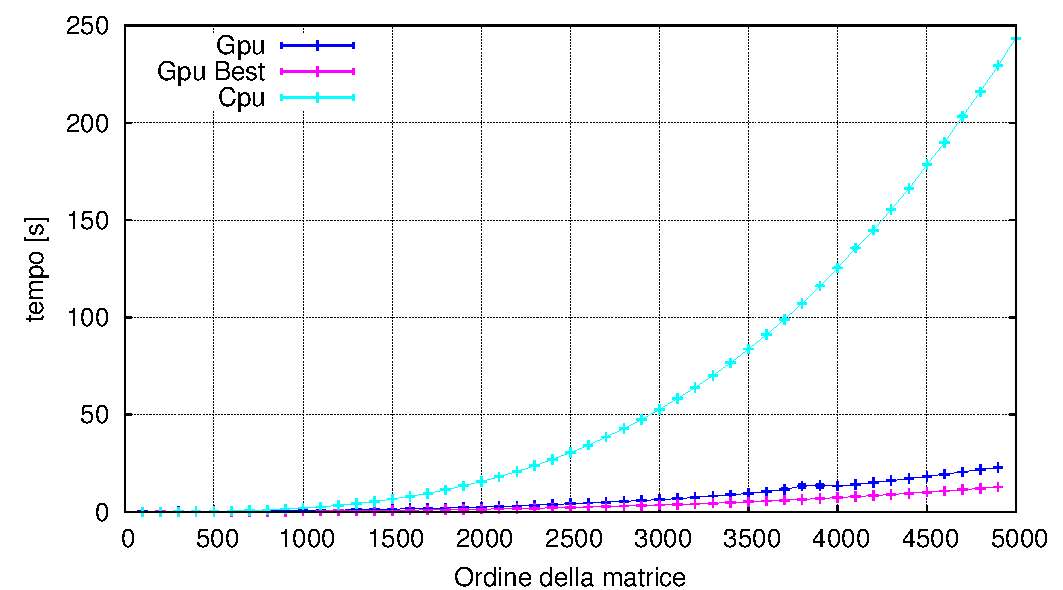
\includegraphics[width=100mm]{TimevsN.pdf}
\end{figure}
\end{frame}

\begin{frame}{Conclusioni}{Confronto tempo d'esecuzione vs Taglia della matrice (zoom)}
\begin{figure}[ht!]
	\centering
	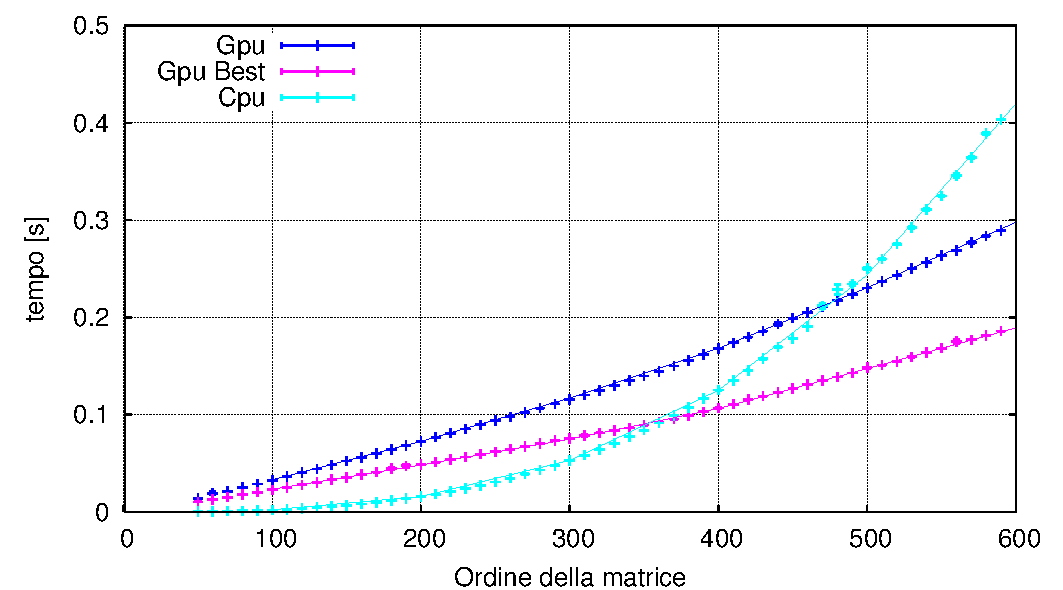
\includegraphics[width=100mm]{TimevsN_Zoom.pdf}
\end{figure}
\end{frame}




\end{document}

